\subsection{Preventing traffic congestions for a one lane road}

Traffic congestion, also known as traffic jams, is when a long line of vehicles moves slowly or has stopped moving altogether. Traffic jams can create frustration, cause more fuel consumption and cause accidents. Many factors can cause traffic congestion, such as:
poorly designed roads, not wide enough roads, traffic light patterns, and accidents \parencite{traffic_congestion}.

With this in mind, we started by focusing on a simple scenario: when a car drastically reduces its speed or completely stops on a single-lane road. 

This scenario will lead to the vehicles behind needing to slow down drastically as well. Because the human reaction is not perfect, this can lead to multiple cars having to emergency brake, disrupting the traffic flow. To prevent this, the vehicles behind have to decrease their velocity before they reach the destination of where the event happened. For this to happen, a server needs to keep track of the positions of the cars and send information to the cars behind when needed. 

After a few discussions, we came up with an idea of how the interactions between the server and the cars would be. First, the car had to connect to the server and give information about its current speed, weight, width, and length. The server would keep track of all the cars positions on the road. There was only one dimension to worry about since there was only a single road. The cars would send information to the server if their velocity changed. This message would trigger an event on the server where it would command all the cars behind the car that triggered the event to slow down accordingly. \figref{fig:diagramfirst} shows a flow chart of a potential demonstration with the cars from the previous group:

\begin{figure}[h!]
	\centering
	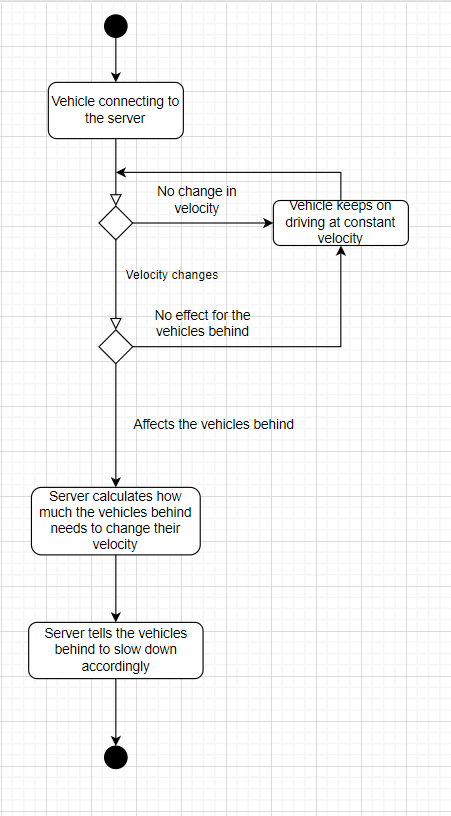
\includegraphics[width=1\linewidth]{figures/flow_diagram_first}
	\caption[Flow diagram server]{Flow diagram for the demo for the first solution.}
	\label{fig:diagramfirst}
\end{figure}